\section{Analyse}
\label{sec:sha256:analyse}

In dieser Analyse geht es um eine oberflächliche Betrachtung der Rundenfunktion und der Kompressionsfunktion.
Ziel ist es ein Verständnis dafür zu entwickeln, was eine Umkehrung der Berechnung verhindert und welche Folgen es
hätte, wenn die Berechnungen gelingt.

\subsection{Rundenfunktion}
\label{sec:ana:rundenfunktion}
In Abbildung \ref{fig:sha256coreA} ist noch einmal die Rundenfunktion mit einigen Markierungen dargestellt.
Bei dem Versuch, die Funktion umzukehren, ist sofort ersichtlich, dass A bis C und E bis G direkt übernommen werden können.

\begin{figure}[!h]
  \centering
  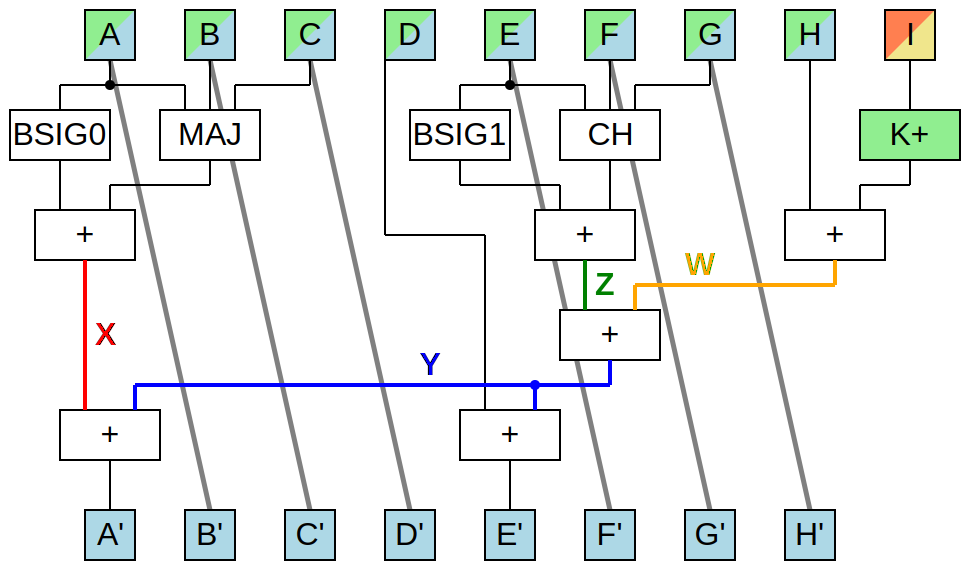
\includegraphics[scale=0.4]{images/sha256coreA}
  \caption{Analyse einer \glos{sha256}-Runde}
  \label{fig:sha256coreA}
\end{figure}

Dadurch lassen sich auch \textcolor{red}{\textbf{X}} und \textcolor{Strong Green}{\textbf{Z}} direkt berechnen.
Mit Hilfe von \textcolor{red}{\textbf{X}} lässt sich schließlich \textcolor{blue}{\textbf{Y}} berechnen, was zu D führt.
Formell ist dieser Zusammenhang in Abbildung \ref{eq:calcD} dargestellt.

\begin{figure}[!h]
  \begin{tabbing}
    XXXXXXXXXXXXXXXXXXXXX\=XX\=XX\=XXXXXX\=XXXX\=XX\=XX\=XXXXXXXX \kill
    \>A'\>=\>\textcolor{red}{\textbf{X}} + \textcolor{blue}{\textbf{Y}}\>$\Rightarrow$\>\textcolor{blue}{\textbf{Y}}\>=\>A' - \textcolor{red}{\textbf{X}}\\
    \>E'\>=\>D + \textcolor{blue}{\textbf{Y}}\>$\Rightarrow$\>\textcolor{blue}{\textbf{Y}}\>=\>E' - D\\
    \>~\\
    \>\>\>E' - D\>=\>A' - \textcolor{red}{\textbf{X}}\\
    \>\>\>-D    \>=\>A' - \textcolor{red}{\textbf{X}} - E'\\
    \>\>\>D     \>=\>\textcolor{red}{\textbf{X}} + E' - A'
  \end{tabbing}
  \caption{Berechnung von D}
  \label{eq:calcD}
\end{figure}

Schließlich lässt sich auch \textcolor{orange}{\textbf{W}} berechnen (\textcolor{blue}{\textbf{Y}} - \textcolor{Strong Green}{\textbf{Z}}). Ab diesem Punkt ist
es jedoch nicht möglich weiter zu rechnen. Da weder H noch I bekannt sind, gibt es $2^{32}$ Möglichkeiten die Summe \textcolor{orange}{\textbf{W}} zu bilden.

\subsection{Urbildberechnung}
\label{sec:urbildberechnung}
Ausgehend davon, dass das Ergebnis von \glos{sha256} eine Länge von 256 Bit hat, und die Eingabe bei einer einzelnen Anwendung der Kompressionsfunktion bis zu
447 Bit lang werden kann, ist es wahrscheinlich, dass jeder \glos{hash} durch eine einzelne Anwendung der Kompressionsfunktion erzeugt werden kann. Um mit vollständigen
Bytes zu arbeiten, wird in diesem Angriffsvektor versucht eine Eingabe mit 440 Bit zu finden. Im Mittel gibt es somit für jeden \glos{hash} $2^{440-256} = 2^{184}$
mögliche Eingaben die jeweils zu einer Kollisionen führen.

Bei einer einzelnen Anwendung der Kompressionsfunktion werden acht Konstanten zum \glos{hash} entwickelt. Da diese bekannt sind und der \glos{hash} ebenfalls vorgegeben ist,
lässt sich die abschließende Addition berechnen (siehe Abbildung \ref{fig:sha256single}). Dadurch sind A' bis H' der letzten Runden bekannt. Wie im vorherigen
Abschnitt beschrieben, müssen in jeder Runde H's und I's gefunden werden, die zu den vorgegebene Konstanten führen und eine gültige Eingabe bilden. Zu beachten
ist, dass die letzten neun Byte durch das \glos{padding} (siehe Abschnitt \ref{sec:sha256:padding}) vorgegeben sind. Das führt in den Runden 15 und 16 dazu, dass
das I vollständig bekannt ist, während es in der Runde 14 teilweise bekannt ist.

Sollte diese Berechnung gelingen, können auch Eingaben beliebiger Länge erzeugt werden. Dazu kann die Kompressionsfunktion beliebig oft mit einer selbst gewählten Eingabe
ohne \glos{padding} ausgeführt werden. Der daraus resultierende \glos{hash} geht als \glos{initialwert} in die letzte Runde ein, deren Eingabe wie oben beschrieben berechnet werden könnte.

Eine Urbildberechnung würde es somit ermöglichen, zu hinterlegten Passwort-\glospl{hash} gültige Passwörter zu berechnen. Das fälschen einer Signatur eines längeren Dokuments
wäre jedoch noch schwierig, da der letzte Block Eingaben enthalten kann, die im gefälschten Dokument auffallen könnten. Um auch dieses Problem zu lösen, wird der nächste
Ansatz betrachtet.

\subsection{Initialwertberechnung}
\label{sec:initialwertberechnung}
Wie im vorherigen Abschnitt zu sehen, kann die Urbildberechnung auf eine einzelne Ausführung von \glos{sha256} zurückgeführt werden.
Problematisch ist jedoch, dass das Ende der erzeugten Eingabe nicht unbedingt sinnvoll ist. Um auch dieses Problem zu lösen, müssten
die Werte A bis H berechnet werden, wobei der \glos{hash} und die Eingabe gegeben sind. I ist somit in jeder Runde bekannt. Da aber die Initalwerte
von A bis H fehlen, ist es nicht mehr möglich, die abschließende Addition zu berechnen, so dass A' bis H' in Runde 64 unbekannt sind. Lediglich
die Differenz zwischen den \glos{initialwert}{en} der ersten Runde und A' bis H' der letzten Runde ist bekannt. Somit ist auch in diesem Fall eine
einfache Berechnung nicht möglich.

Sollte diese Berechnung gelingen, wäre es möglich, ein Dokument zu erstellen, dass neben einem frei gewählten Inhalt zum Beispiel eine ausgeblendete
Grafik oder einen sichtbaren QR-Code enthält. Die Hash-Berechnung könnte dann bis inklusive der einleitenden Bilddaten durchgeführt werden.
Die abschließenden Bilddaten und das Dokumentende würden als Eingabe für die letzte Ausführung dienen, für die der \glos{initialwert} berechnet wird.
Für die vorletzte Ausführung, die die Bilddaten verarbeitet, müsste so eine Urbildberechnung durchgeführt werden, für die keinerlei Anforderungen
an die Eingabe gestellt werden braucht.

\subsection{Kollisionsberechnung}
\label{sec:kollisionsberechnung}
Im Gegensatz zu den Berechnungen in den beiden vorigen Abschnitten hat die Kollisionsberechnung keine praktische Anwendung, da keine Anforderung an
den \glos{hash} gestellt sind. Ziel ist es lediglich 2 beliebige Eingaben zu finden, die zu einem gleichen \glos{hash} führen. Mit Hilfe eines SAT-Solvers
(siehe Abschnitt \ref{sec:satsolver}) lässt dich dieses Problem einfach formulieren. Dazu werden 2 Instanzen des Hash-Algorithmus in den SAT-Solver eingefügt
und in einer Miter-Schaltung \cite{mitergraph} verknüpft. In dieser Schaltung werden die Ausgänge (Hahes) gleichgesetzt und ein Unterschied in mindestens
einem Eingabebit gefordert. So kann der SAT-Solver nach einer Lösung suchen ohne dass ein \glos{hash} vorgegeben wurde. Das Geburtstagsparadoxon findet somit
praktische Anwendung.